\chapter{Diseño}

\section{Introducción}

\newpage

%\section{Diagrama de Clases de Análisis}

%\newpage

\section{Diagrama de Clases}

\begin{figure}[th!]
	\centering
	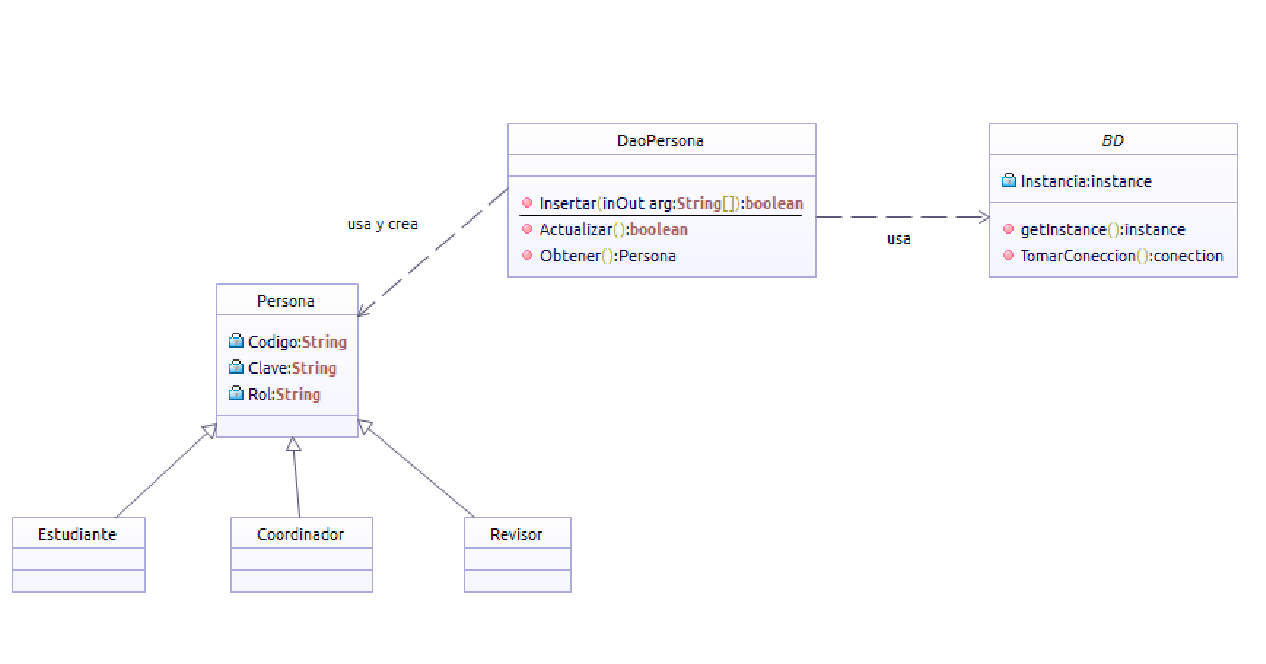
\includegraphics[width=1.2\linewidth]{uml/Clases/ClasesCrearUsuario}
	\caption{Registrar Usuario}
	\label{fig:Registrar Usuario}
\end{figure}

\newpage

\section{Patrones}

\subsection{Creacionales}

\bigskip

\subsubsection{Builder}

\begin{figure}[th!]
	\centering
	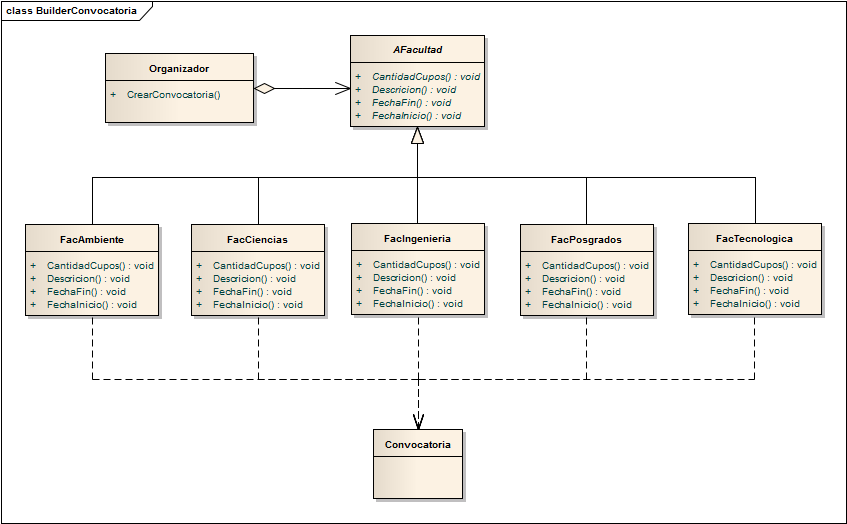
\includegraphics[width=1.2\linewidth]{uml/Patrones/BuilderConvocatoria}
	\caption{Builder para crear convocatoria}
	\label{fig:Builder para convocatoria}
\end{figure}



\subsection{Factory}

\begin{figure}[th!]
	\centering
	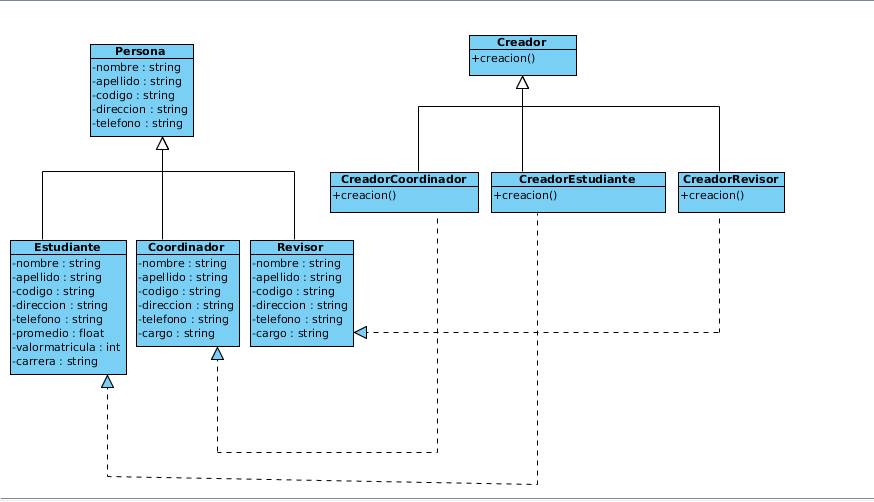
\includegraphics[width=1.2\linewidth]{uml/Patrones/FactoryMethod}
	\caption{Factory para crear personas}
	\label{fig:Factory}
\end{figure}

\newpage

\subsection{Estructurales}

\subsection{Comportamiento}

%\section{Diagrama de Objetos}

%\newpage

%\section{Diagrama de Estructura Compuesta}

%\newpage